\section{Requisiti Front-End}
\label{sec:RequisitiFrontEnd}

Nel presente capitolo vengono riportati alcuni mockup relativi alle schermate dell’applicazione per Web da realizzare. Queste schermate hanno l’obiettivo di rappresentare come l’applicazione si dovrà presentare all’utente finale, il front end (FE), nel caso dei seguenti requisiti funzionali descritti precedentemente: 
\begin{itemize}
    \item registrazione e login nella piattaforma (\ref{rf:1.1})
    \item interazione con calendari di altre persone (\ref{rf:4.1});
    \item compilazione/modifica evento (\ref{rf:5});
    \item impostazione impegno (\ref{rf:6});
    \item interazione con un servizio di mappe (\ref{rf:8.2});
    \item riorganizzazione di attività (\ref{rf:10});
    \item informazioni sull’uso del tempo (\ref{rf:9});
\end{itemize}

\begin{listaPersonale}{FE}
    \elemento[LOGIN NELLA PIATTAFORMA]{fe:1} In questa schermata, l’utente già registrato mediante email e password, deve inserire le credenziali da lui scelte per accedere al sito. Invece, coloro che hanno fatto accesso grazie all’utilizzo di servizi di terze parti, devono proseguire la loro autenticazione premendo il tasto corrispondente al servizio esterno da loro utilizzato per registrarsi (\ref{rf:1.1}).
    Se l’utente non si è ancora registrato sul sito deve schiacciare “Registrati” oppure proseguire l’autenticazione con uno dei servizi di terze parti offerti, ovvero Google ed Apple.
    \begin{figure}[H]
        \centering
        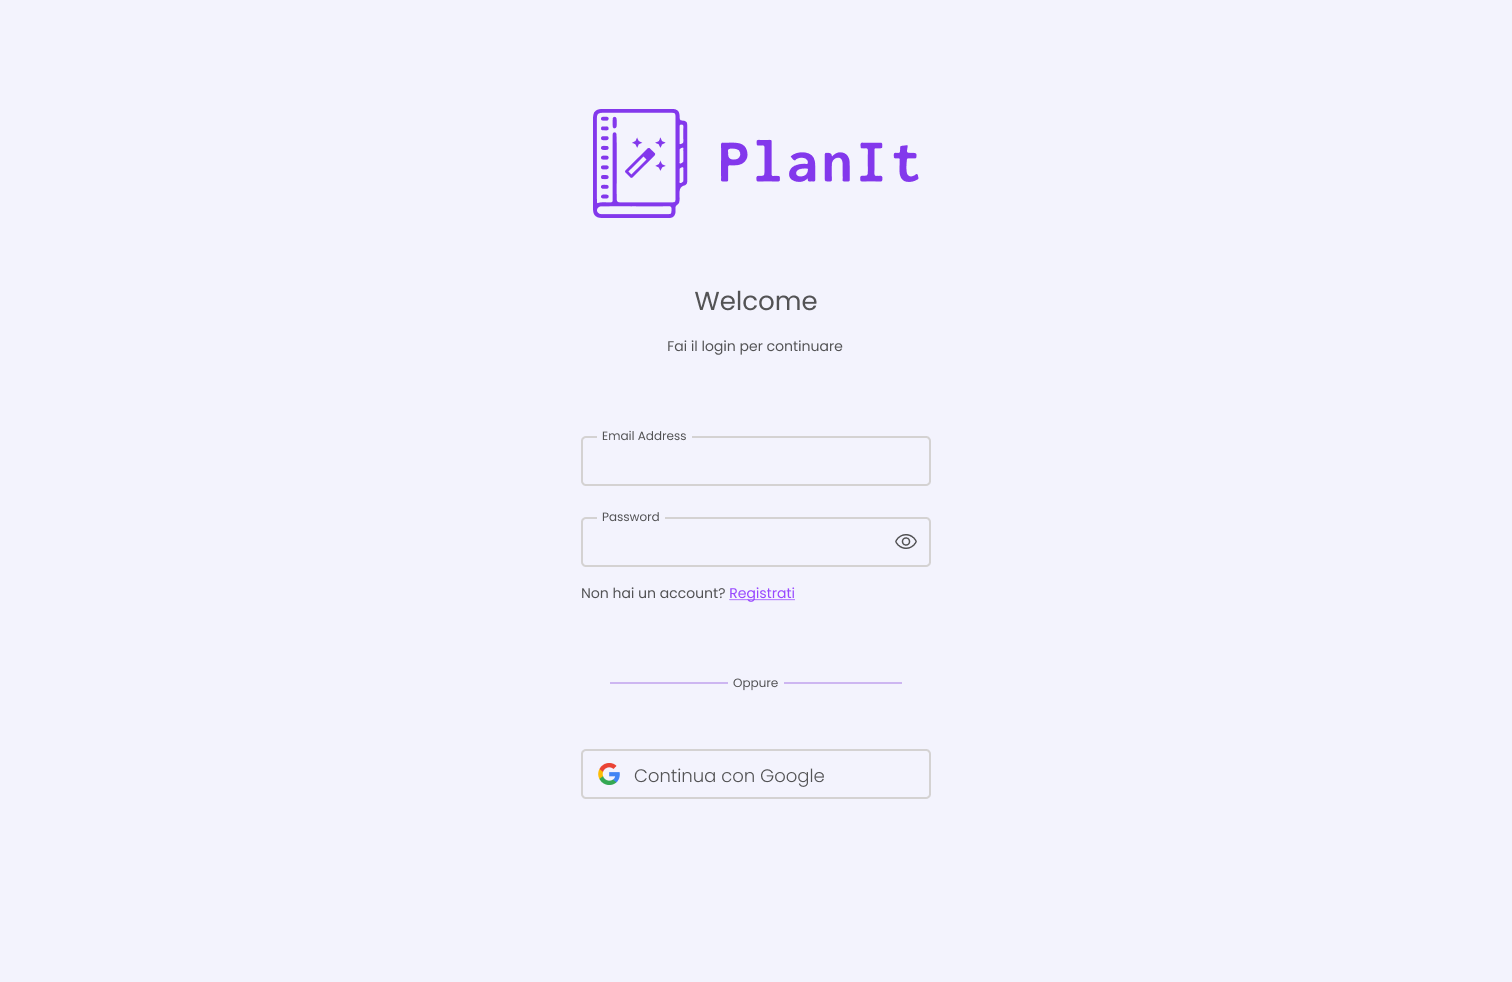
\includegraphics[width=1\textwidth]{img/FrontEnd/Login.png}
        \caption{Figura 1: schermata quando si apre il sito PlanIt}
    \end{figure}
    \begin{listaPersonale2}{FE}
        \elemento[SCHERMATA RESET PASSWORD]{fe:1.1}
        \begin{figure}[H]
            \centering
            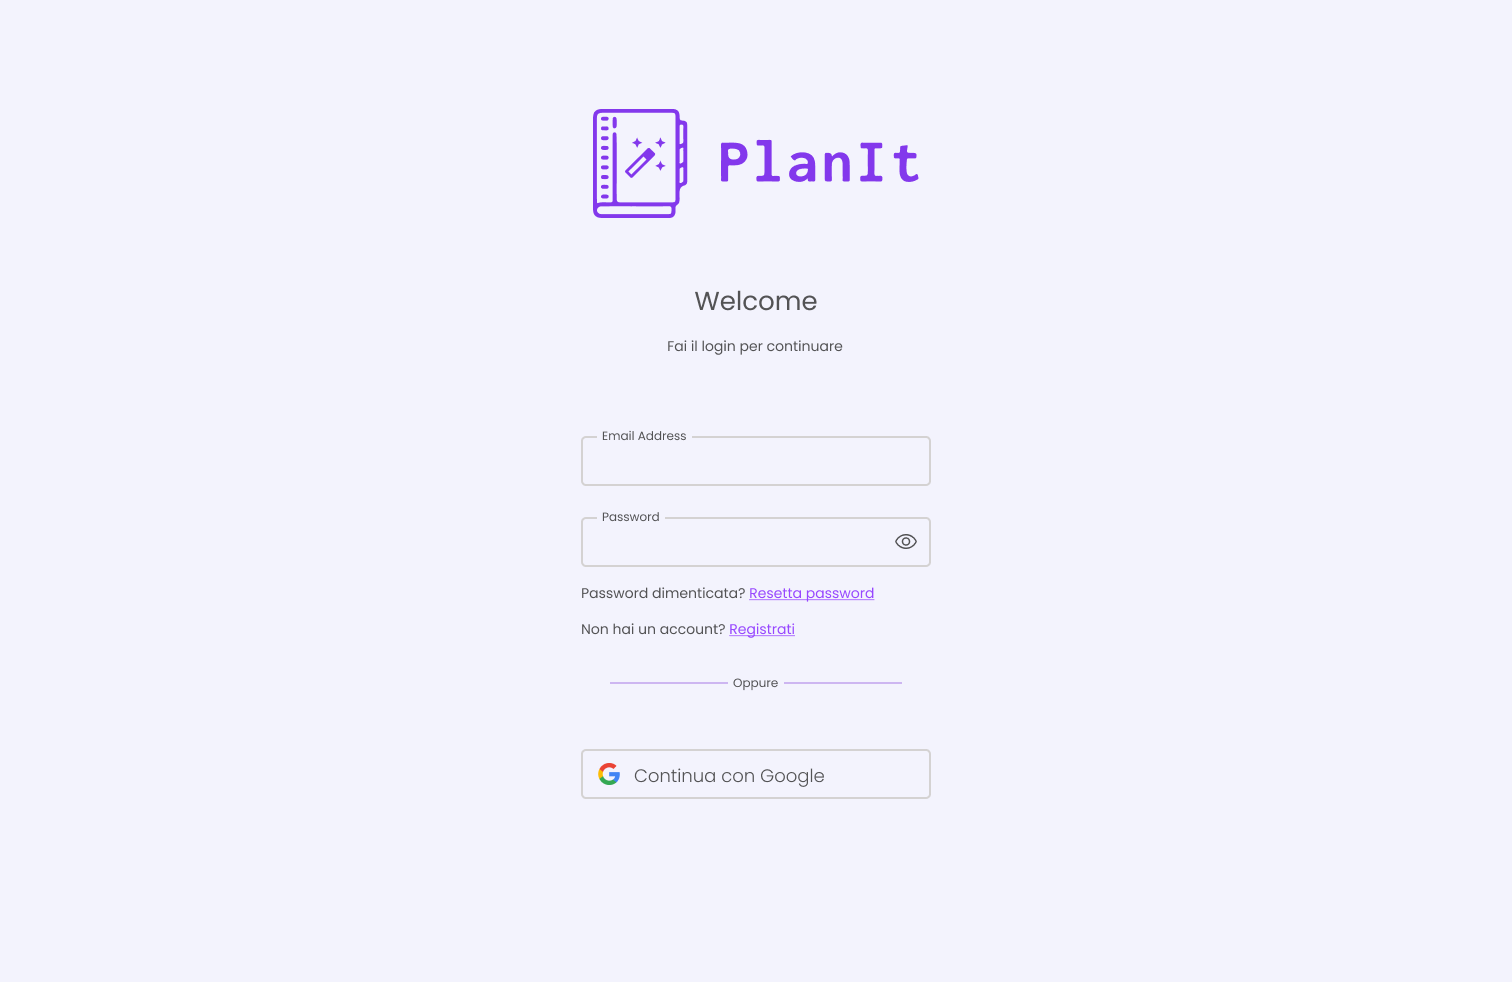
\includegraphics[width=1\textwidth]{img/FrontEnd/ResettaPssw.png}
            \caption{Figura 1.1: schermata che appare quando si sbaglia più volte una password (\ref{rf:15})}
        \end{figure}
    \end{listaPersonale2}

    \pagebreak%quasi quasi metterei un pagebreak per ciascuna schermata così per renderlo più ordinato
    
    \elemento [SCHERMATA PRINCIPALE] {fe:2} Questa schermata è la schermata principale della piattaforma PlanIt. L’utente, dopo aver fatto l’accesso al sito oppure proseguito con la modalità demo, giungerà a questa pagina, dove potrà guardare gli eventi posti nella settimana. L’utente ha la possibilità, dal menù al di sopra del calendario, di spostarsi di data sia in mesi che in settimane e accedere agli altri calendari personali e a quelli condivisi (\ref{rf:4.1}). Infine è presente anche il bottone "+” con cui si accede al pop-up di compilazione/aggiunta evento(\ref{rf:5}).
    \begin{center}
        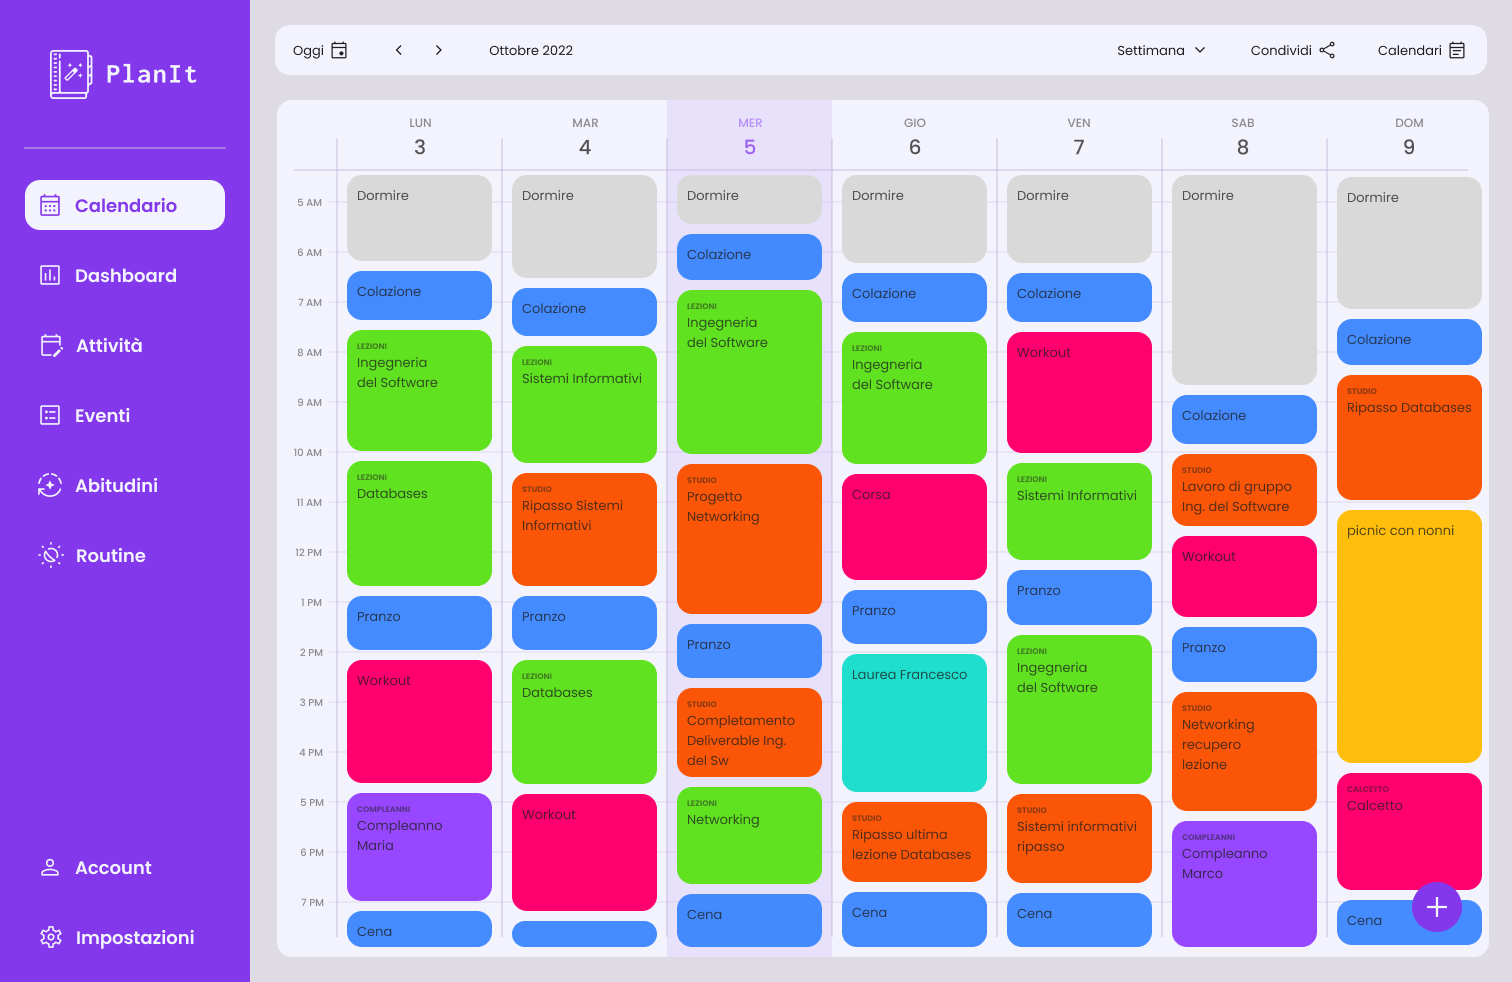
\includegraphics[width=1\textwidth]{img/FrontEnd/Calendar/Calendar.png}
    \end{center}
    
    \begin{listaPersonale2}{FE}
        \elemento[SCHERMATA PRINCIPALE-CALENDARI]{fe:2.1} Grazie alla sezione “Calendari” l’utente aprirà una sezione da dove può gestire i propri calendari, divisi per tematiche, e i calendari condivisi di altre persone (\ref{rf:4.1}). I calendari condivisi sono indicati con una piccola immagine stereotipata di persona, alla destra del loro nome.
    \end{listaPersonale2}
    \begin{center}
        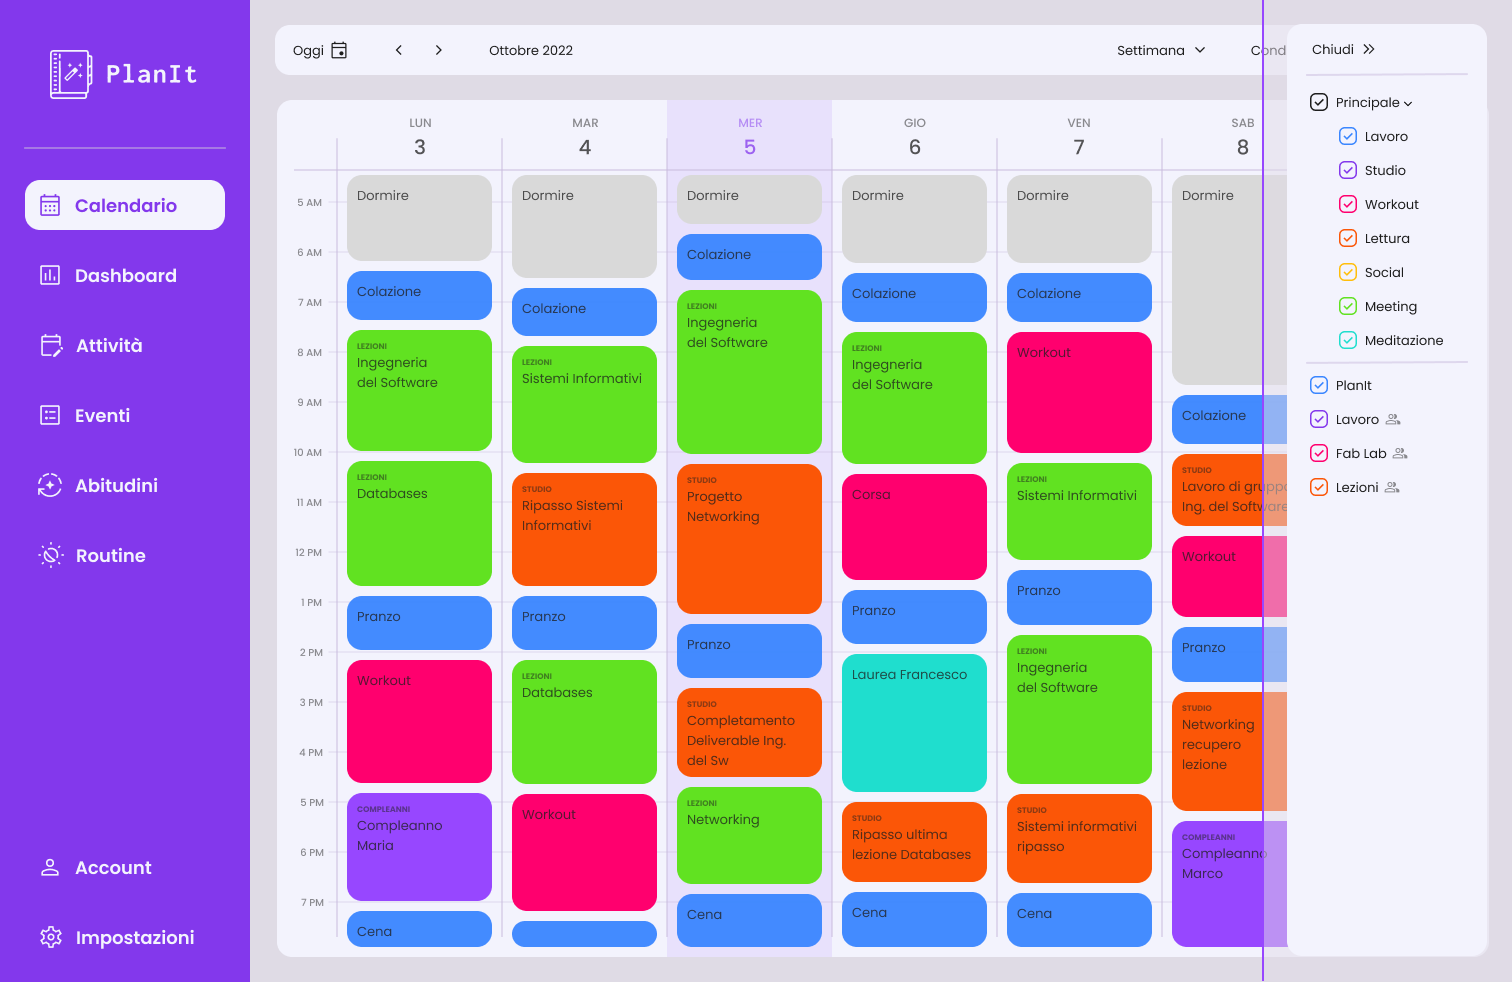
\includegraphics[width=0.85\textwidth,height=0.30\textheight]{img/FrontEnd/Calendar/CalendarCondivisi.png}
    \end{center}

    \pagebreak
    \elemento[DASHBOARD] {fe:3} L’utente, nella dashboard, può osservare le informazioni principali riguardo al proprio calendario, le sezioni presenti sono: attività svolte questa settimana, situazione scadenza attività e attività svolte oggi con grafico attività svolte.
    \begin{center}
        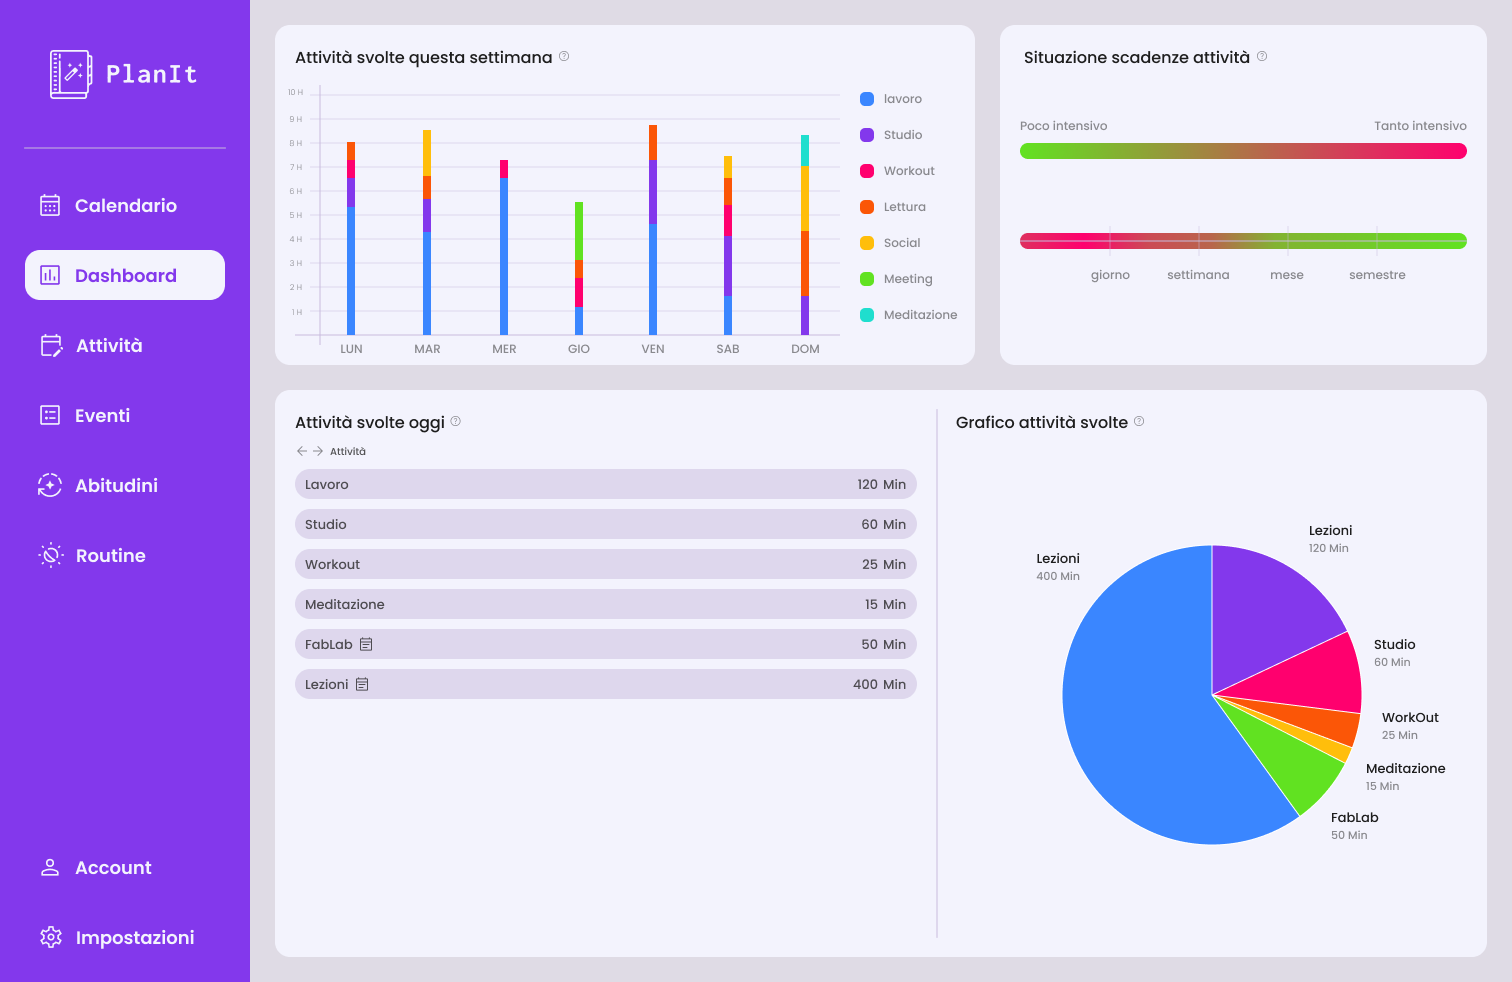
\includegraphics[width=1\textwidth]{img/FrontEnd/Dashboard/Dashboard.png}
    \end{center}
    
    \begin{listaPersonale2}{FE}
        \elemento[ATTIVITA' SVOLTE QUESTA SETTIMANA] {fe:3.1} Nella sezione “Attività svolte questa settimana” viene mostrato un grafico a barre delle varie attività svolte per ogni giorno della settimana (\ref{rf:9}), l’altezza delle barre corrisponde al quantitativo di ore dedicate a quell’attività.

        \begin{center}
            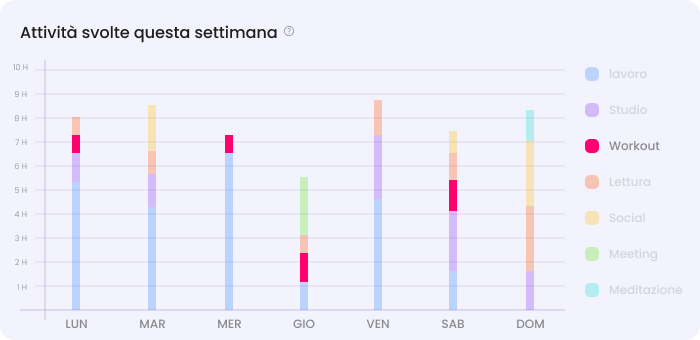
\includegraphics[width=0.6\textwidth,height=0.18\textheight]{img/FrontEnd/Dashboard/graficoBarre.png} %questa vorrei che fosse una wrap figure
        \end{center}
        \pagebreak
        \elemento[SITUAZIONE SCADENZA ATTIVITA'] {fe:3.2}
        Nella sezione “Situazione scadenze attività” è presente in basso una heatmap riguardo al tempo che deve essere dedicato ogni giorno per rispettare le varie deadline (\ref{rf:9}). La legenda sopra la heatmap mostra che più è tendente il colore al rosso, più ore devono essere impiegate nello specifico periodo di tempo.
        \begin{center}
            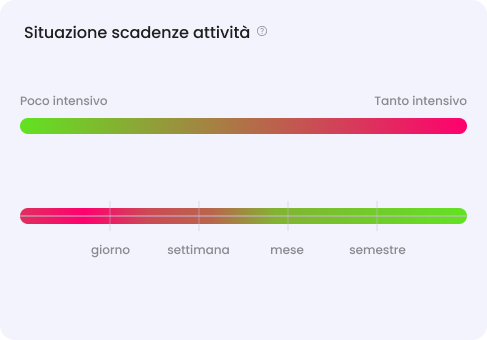
\includegraphics[width=0.45\textwidth,height=0.18\textheight]{img/FrontEnd/Dashboard/heatMap.png} %questa vorrei che fosse una wrap figure
        \end{center}

        
        \elemento [ATTIVITA’ SVOLTE OGGI e GRAFICO ATTIVITA' SVOLTE] {fe:3.3} Nella sezione “Attività svolte oggi” è presente una lista delle attività della giornate, da cui si possono ottenere anche le varie sottoattività. 
        La sezione “Attività svolte oggi” è sincronizzata con il grafico a torta presente nel “Grafico attività svolte” (\ref{rf:9}). Il grafico presenta le attività selezionate in “Attività svolte oggi” con una dimensione proporzionata al tempo da spendere.

        \begin{figure}[H]
            \centering
            \includegraphics[width=0.72\textwidth,height=0.2\textheight]{img/FrontEnd/Dashboard/selezionatoAttività.png}
            \caption{Figura 3.3.1: schermata che appare quando si mette il puntatore sopra una delle attività della lista}
        \end{figure}

        \begin{figure}[H]
            \centering
            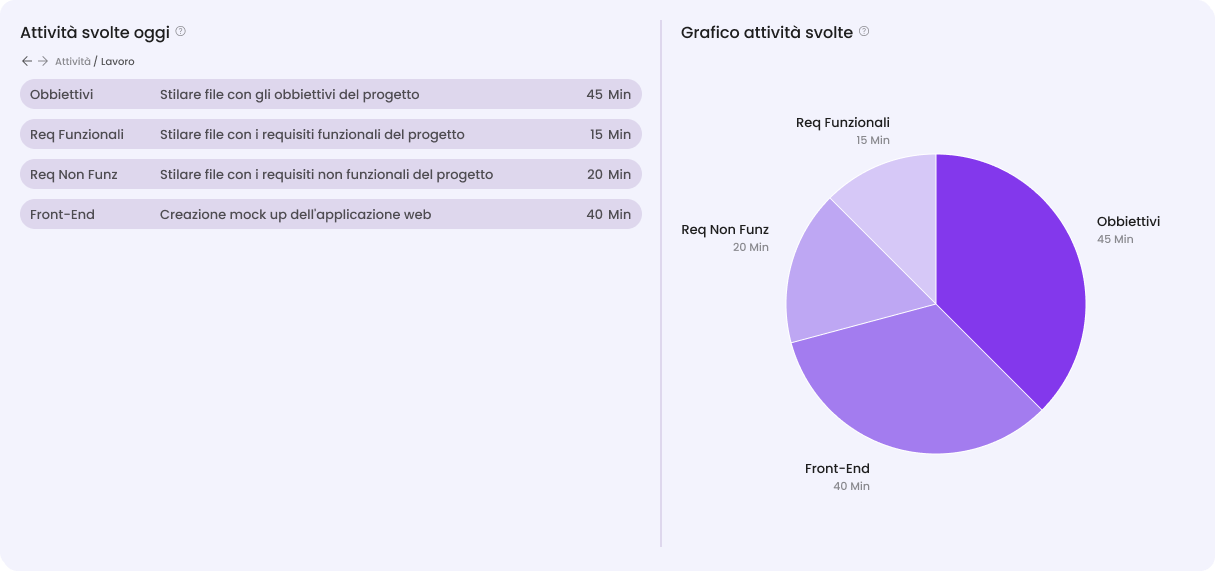
\includegraphics[width=0.72\textwidth,height=0.2\textheight]{img/FrontEnd/Dashboard/Dashboard3.png}
            \caption{Figura 3.3.2: schermata quando si seleziona una delle attività della lista}
        \end{figure}
           
    \end{listaPersonale2}
    \pagebreak
    \elemento [SCHERMATA ATTIVITA'] {fe:4} Nella schermata attività è presente una tabella delle attività della giornata con le varie informazioni, ovvero: titolo, descrizione, categoria, priorità, durata (\ref{rf:5}), posizione (\ref{rf:8.2}). Inoltre ci sono dei tasti con cui si può rimandare e ritardare l’attività (RF10) e, infine, un tasto per indicare di averla completata. A fine giornata di default tutti gli impegni sono posti come completati; per modificare tale opzione deve intervenire l’utente.
    \pagebreak
    \elemento [SCHERMATA EVENTI] {fe:5} Nella schermata eventi sono presenti tutti i comandi che riguardano la compilazione, modifica degli eventi (\ref{rf:5}), creazione di un calendario (\ref{rf:2.2.2}), creazione di raggruppamento di attività ed eliminazione di un evento (\ref{rf:5}).
    Nella sezione sottostante, è presente una lista dei vari calendari e raggruppamenti, che selezionati una alla volta aprono i rispettivi form di modifica e creazione, dove sono presenti tutti i campi citati in RF5 per l’aggiunta e modifica di impegni, RF13 per modifica e aggiunta di calendario. 
    %qua dipende dalla formattazione andrebbe un clearpage
    \begin{figure}[H]
        \centering
        \includegraphics[width=1\textwidth]{img/FrontEnd/Eventi/SottoAttività.png}
        \caption{Figura 5: schermata quando si apre la sezione "Eventi"}
    \end{figure}
    \begin{figure}[H]
        \centering
        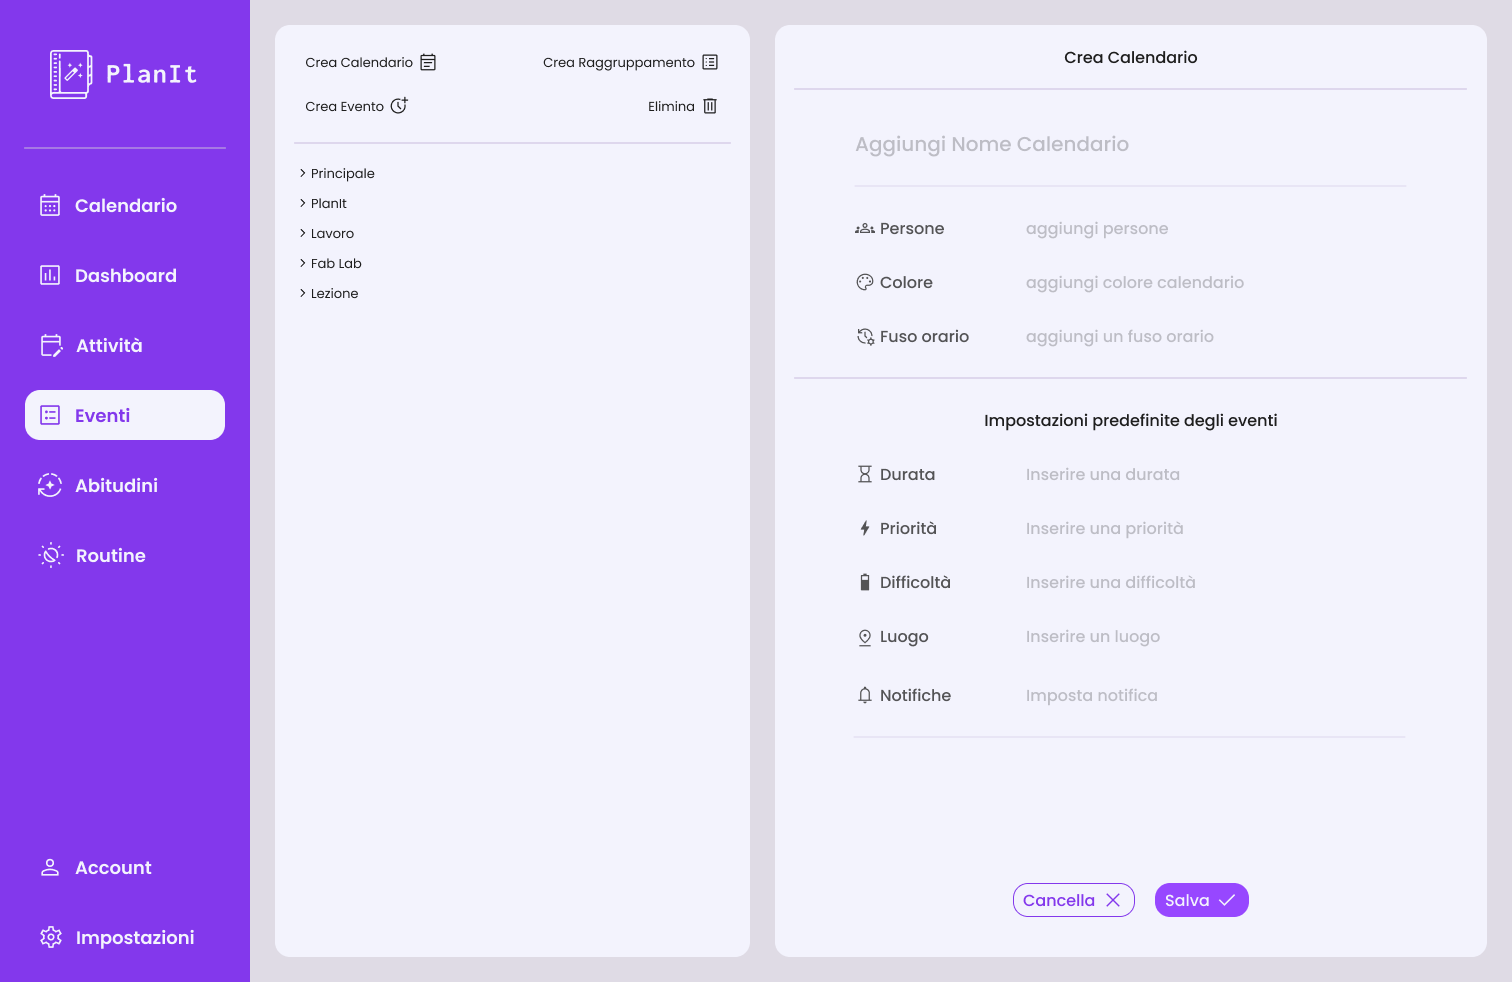
\includegraphics[width=1\textwidth]{img/FrontEnd/Eventi/Calendario/CreaCalendario.png}
        \caption{Figura 5: schermata quando si seleziona uno dei comandi o un'attività della lista}
    \end{figure}
    \begin{listaPersonale2}{FE}
        
        \elemento[SCHERMATA CREA/MODIFICA EVENTO] {fe:5.1}

        \begin{center} 
            \begin{figure}[H]
            \centering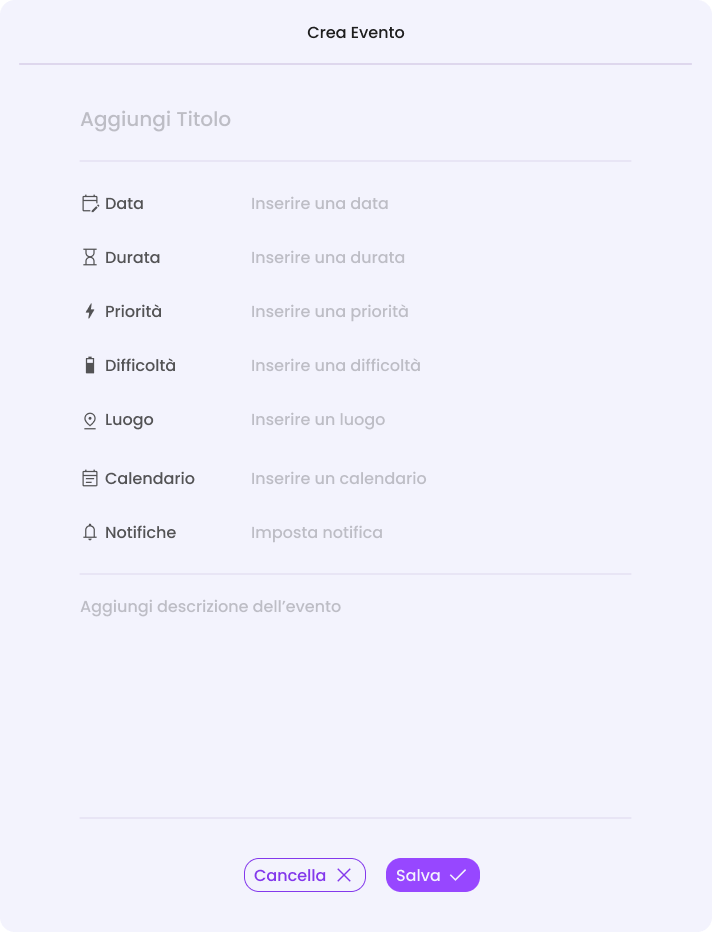
\includegraphics[width=0.49\textwidth,height=0.35\textheight]{img/FrontEnd/Eventi/Evento/CreaEvento.png}
            \centering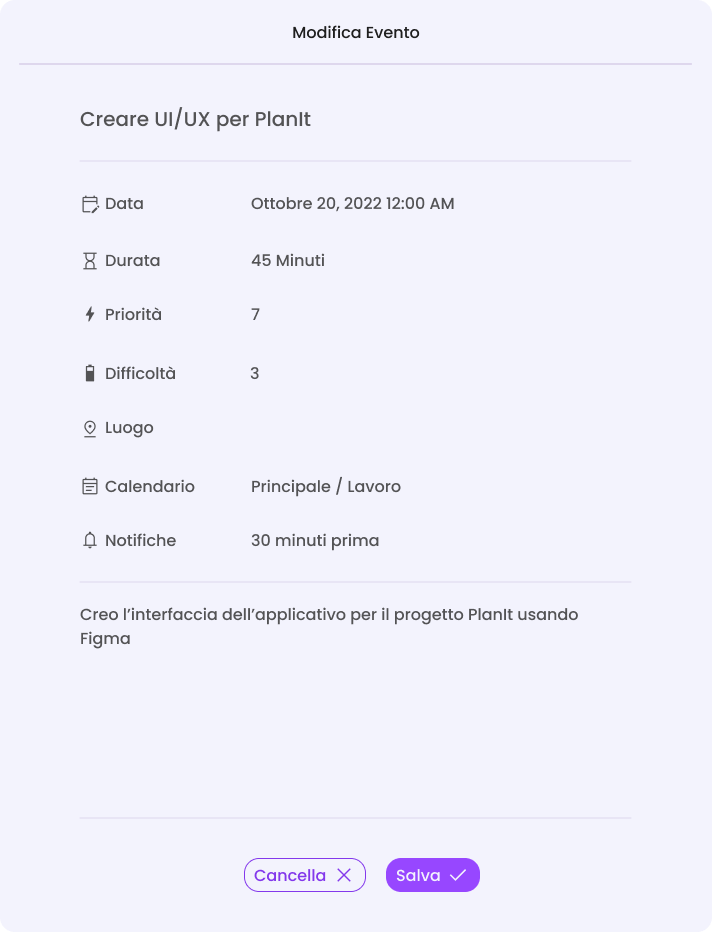
\includegraphics[width=0.49\textwidth,height=0.35\textheight]{img/FrontEnd/Eventi/Evento/ModificaEvento.png}
            \end{figure}
        \end{center}

        
        \elemento[SCHERMATA CREA/MODIFICA RAGGRUPPAMENTO] {fe:5.2}

        \begin{center} 
            \begin{figure}[H]
            \centering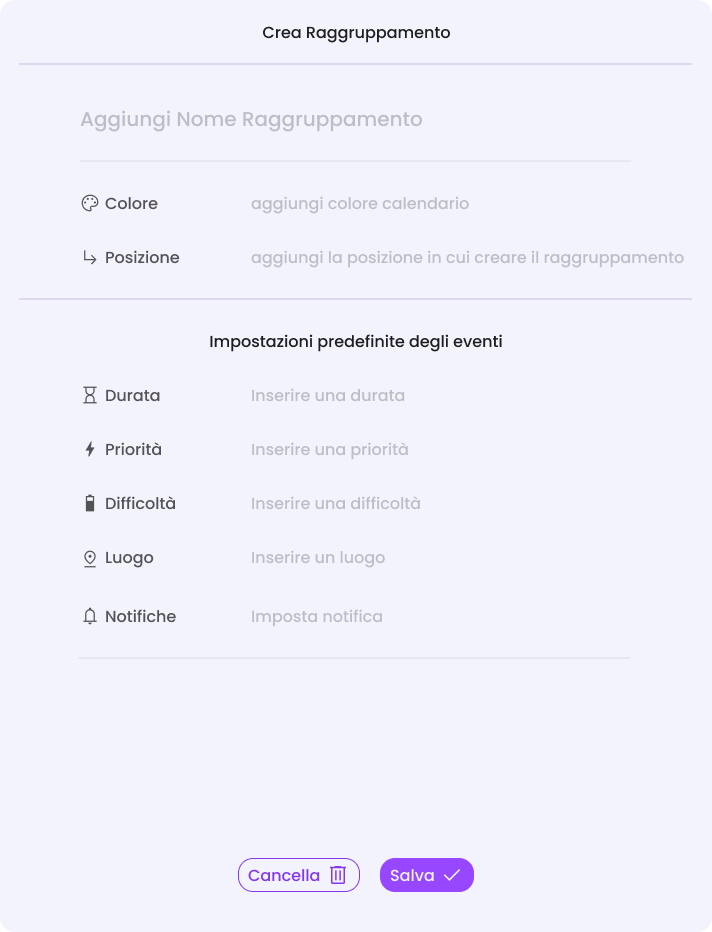
\includegraphics[width=0.49\textwidth,height=0.35\textheight]{img/FrontEnd/Eventi/Raggruppamento/CreaRaggruppamento.png}
            \centering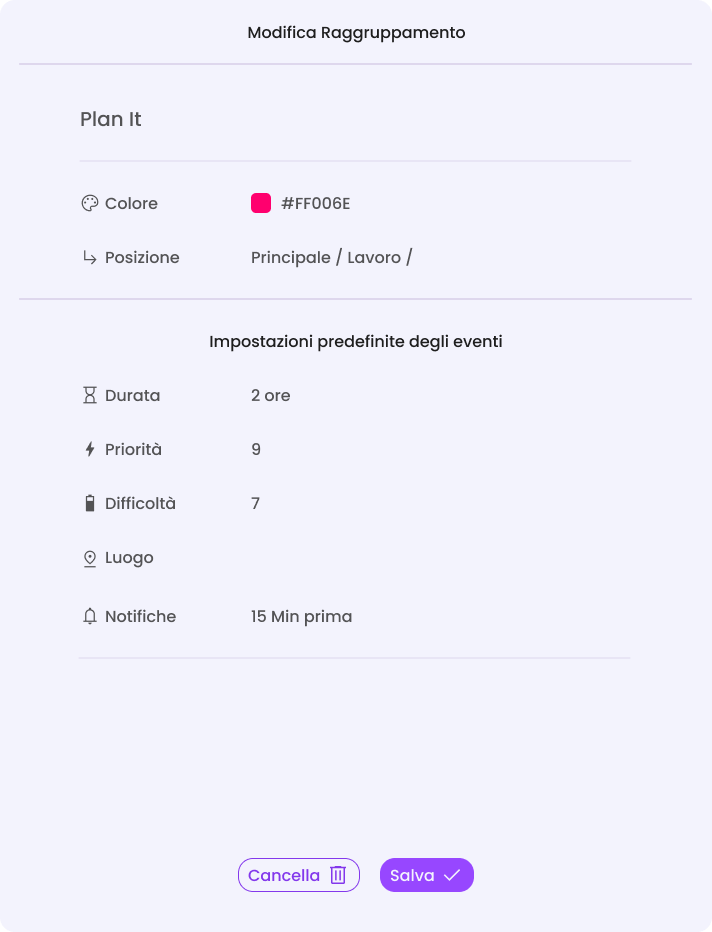
\includegraphics[width=0.49\textwidth,height=0.35\textheight]{img/FrontEnd/Eventi/Raggruppamento/ModificaRaggruppamento.png}
            \end{figure}
        \end{center}
        \pagebreak
        \elemento[SCHERMATA CREA/MODIFICA CALENDARIO] {fe:5.3}

        \begin{center} 
            \begin{figure}[H]
            \centering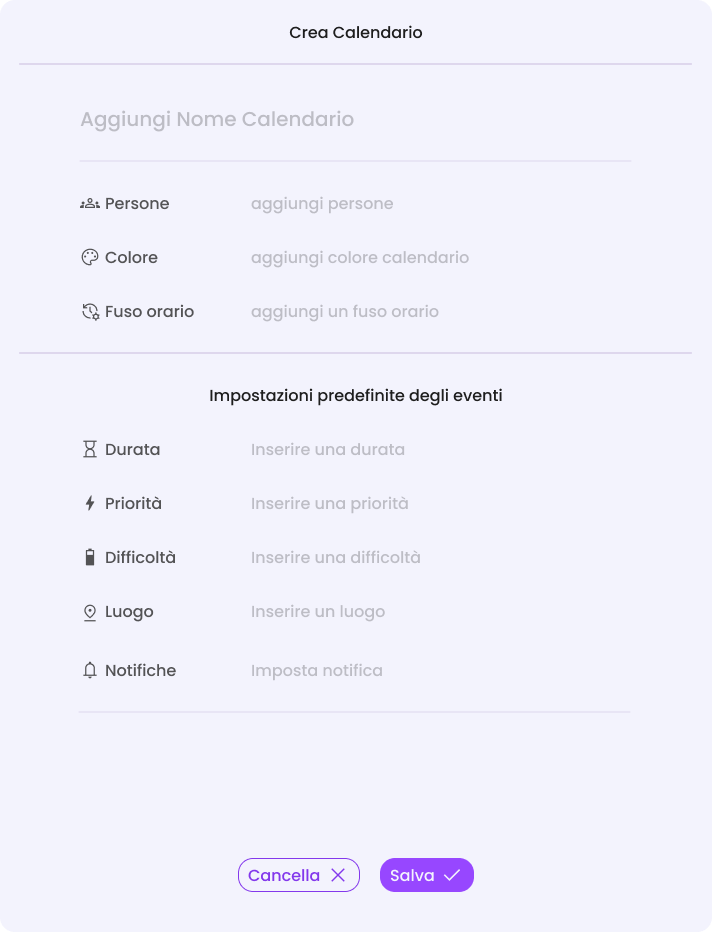
\includegraphics[width=0.49\textwidth,height=0.35\textheight]{img/FrontEnd/Eventi/Calendario/CreaCalendario1.png}
            \centering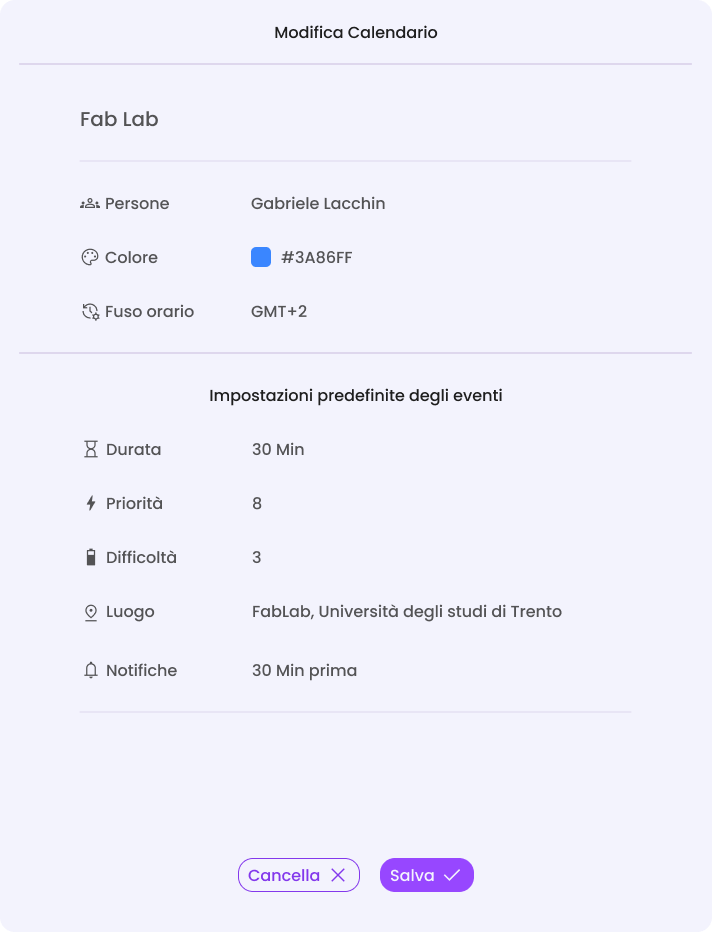
\includegraphics[width=0.49\textwidth,height=0.35\textheight]{img/FrontEnd/Eventi/Calendario/ModificaCalendario.png}
            \end{figure}
        \end{center}
        
    \end{listaPersonale2}
    \pagebreak
    \elemento [SCHERMATA ABITUDINI] {fe:6} Nella schermata “Abitudini”, l’utente può visualizzare la lista delle abitudini del proprio calendario. Inoltre c’è la possibilità di aggiungere, modificare ed eliminare (\ref{rf:5}) le abitudini del proprio calendario, ovvero le attività ripetute in un periodo determinato di tempo (RF, \ref{rf:5.5}), grazie alla sezione che si trova alla destra, dove si apre un form quando si va ad aggiungere e modificare un’ abitudine.

    \begin{figure}[H]
        \centering
        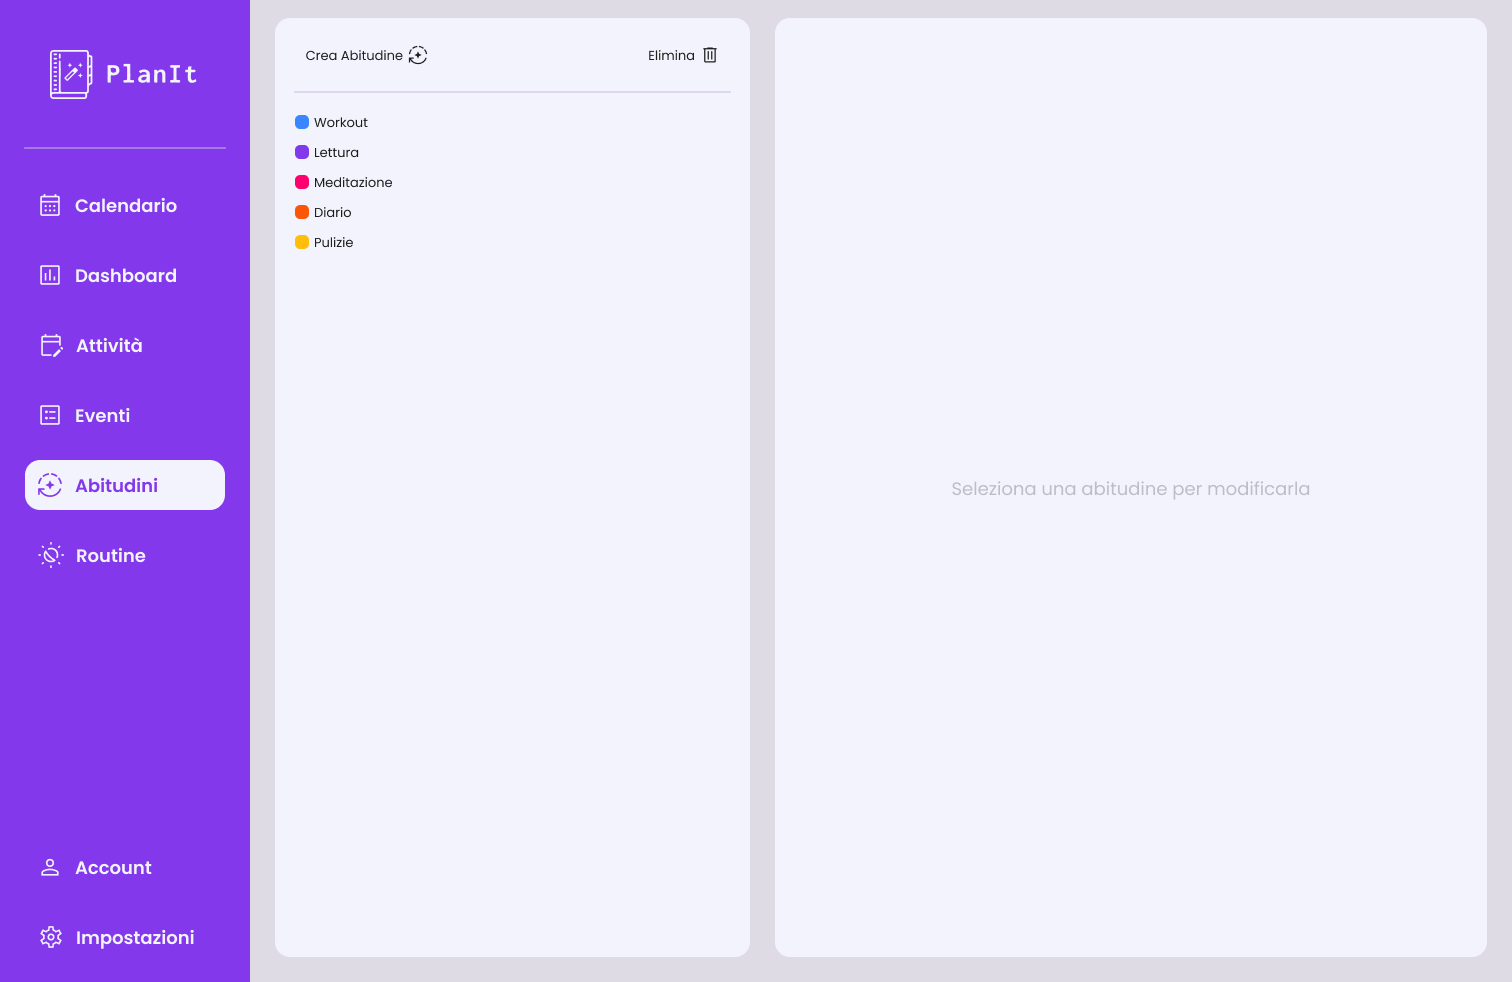
\includegraphics[width=1\textwidth]{img/FrontEnd/Abitudini/Abitudini.png}
        \caption{Figura 6: schermata quando si apre la sezione "Abitudini"}
    \end{figure}

    \begin{figure}[H]
        \centering
        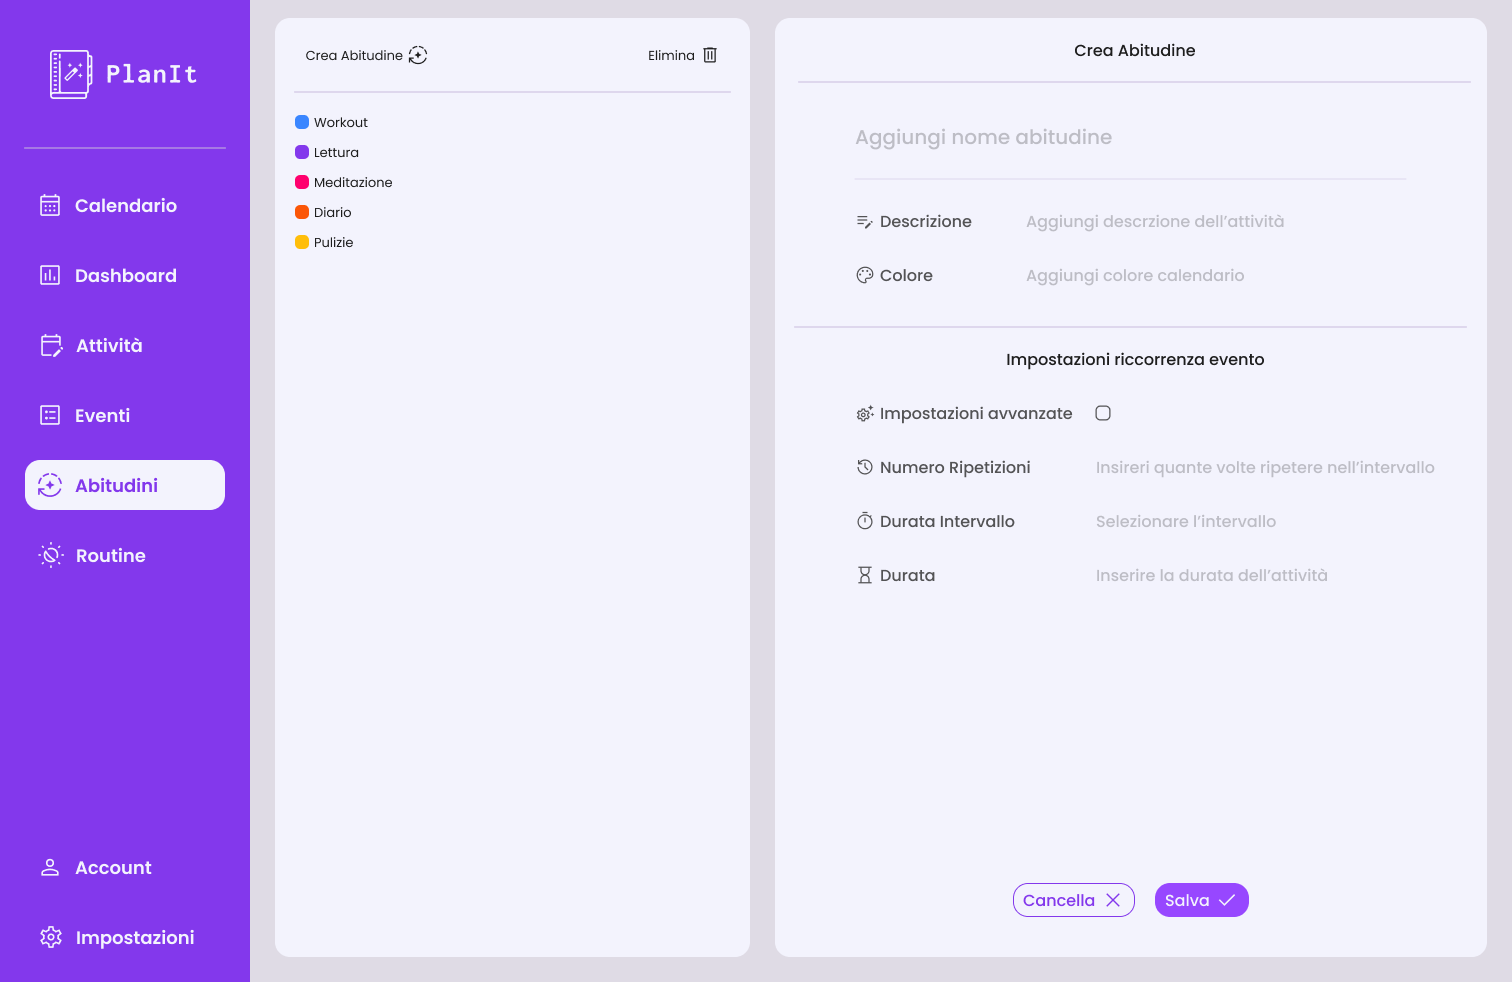
\includegraphics[width=1\textwidth]{img/FrontEnd/Abitudini/CreaAbitudiniMain.png}
        \caption{Figura 6: schermata quando si seleziona uno dei comandi o un'abitudine della lista}
    \end{figure}

    \begin{listaPersonale2}{FE}
        
        \elemento[SCHERMATA CREA ABITUDINI E IMPOSTAZIONI AVANZATE]{fe:6.1}
        \begin{center} 
            \begin{figure}[H]
            \centering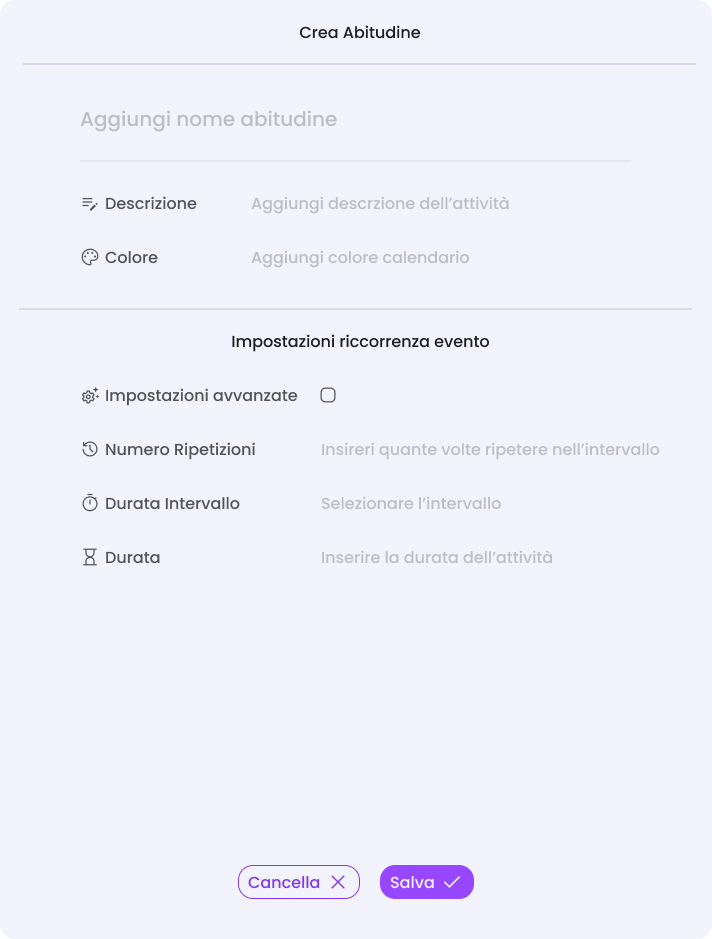
\includegraphics[width=0.49\textwidth,height=0.35\textheight]{img/FrontEnd/Abitudini/Crea/CreaAbitudine.png}
            \centering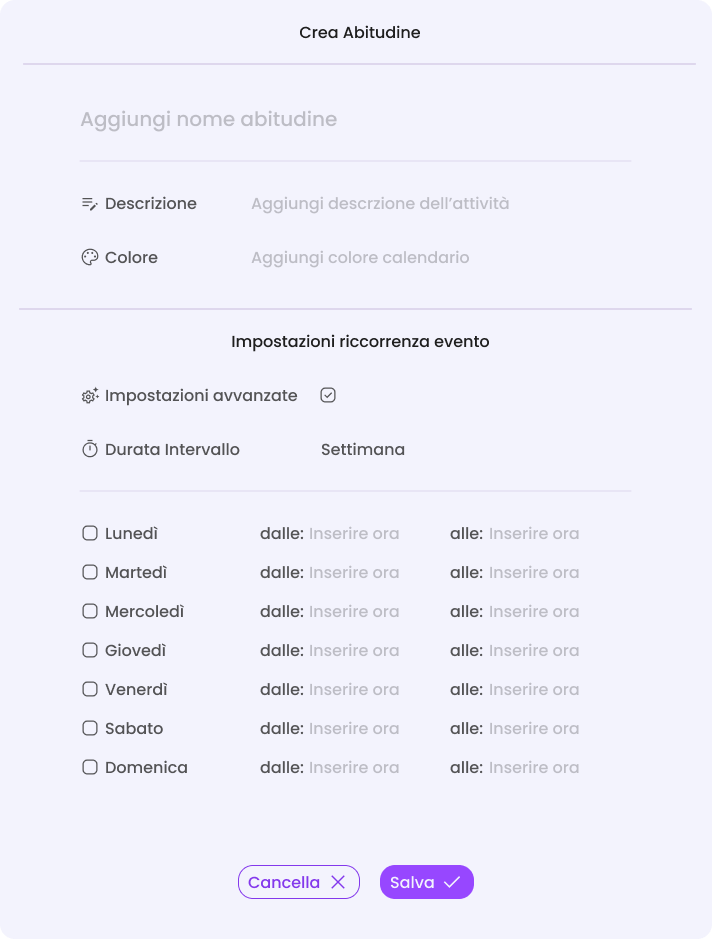
\includegraphics[width=0.49\textwidth,height=0.35\textheight]{img/FrontEnd/Abitudini/Crea/CreaAbitudineAvv.png}
            \end{figure}
        \end{center}

        \elemento [SCHERMATA MODIFICA ABITUDINI E IMPOSTAZIONI AVANZATE] {fe:6.2}
        \begin{center} 
            \begin{figure}[H]
            \centering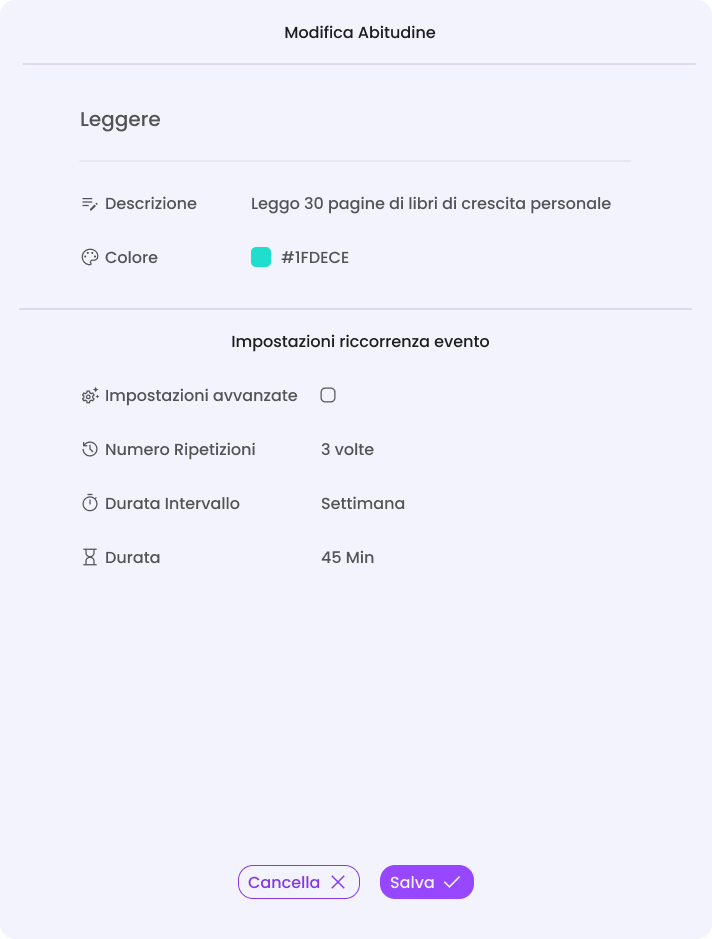
\includegraphics[width=0.49\textwidth,height=0.35\textheight]{img/FrontEnd/Abitudini/Modifica/ModificaAbitudine.png}
            \centering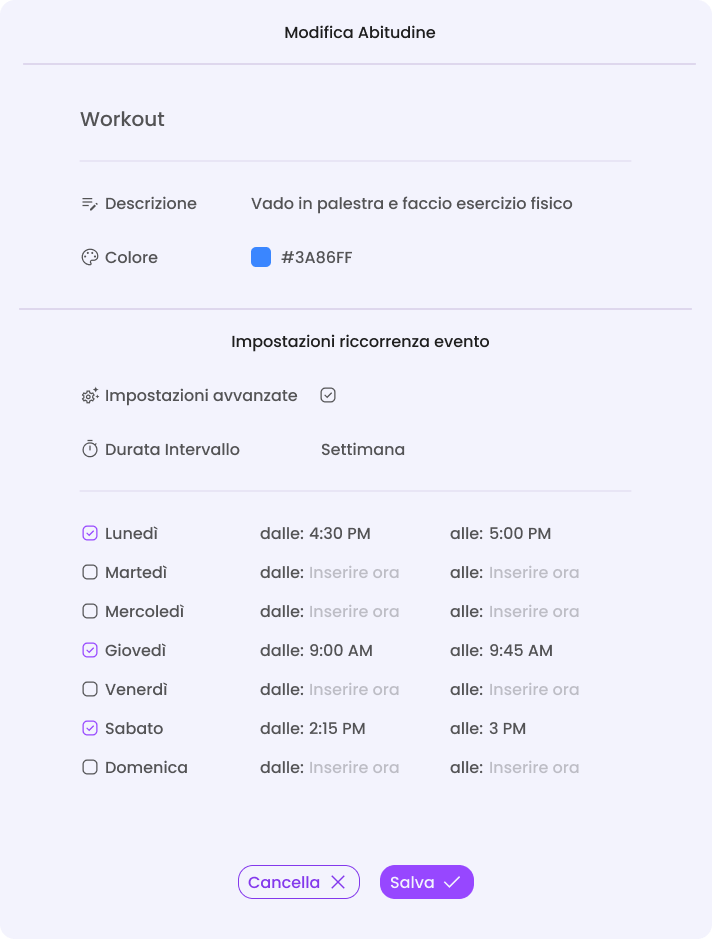
\includegraphics[width=0.49\textwidth,height=0.35\textheight]{img/FrontEnd/Abitudini/Modifica/ModificaAbitudineAvv.png}
            \end{figure}
        \end{center}

    \end{listaPersonale2}
    \pagebreak

    \elemento [SCHERMATA ROUTINE] {fe:7} Nella schermata “Routine” l’utente ha possibilità di visualizzare e gestire tutte le proprie routine, ovvero attività che ripete tutti i giorni (RF,\ref{rf:5.5}), come dormire, mangiare e lavorare. L’utente ha la possibilità di definire quante ore e quando avere queste attività di routine, oppure lasciare al sistema di definire da solo quando avere quell’evento seguendo le regole definite in \ref{rf:6}.
    

\end{listaPersonale}


(Inoltre i cookie saranno usati per mantenere l'accesso così da evitare di fare il login ogni volta che si vuole utilizzare la piattaforma.)